\RequirePackage{fix-cm}
\documentclass[11pt,a4paper]{article}

% Layout and section hierarchy from the II2202 final-report template (2026).
% Compile with LuaLaTeX, BibTeX, then LuaLaTeX twice.
\usepackage[margin=1in,headheight=15pt,headsep=24pt,footskip=28pt]{geometry}
\IfFileExists{sourcesans.sty}
  {\usepackage[default]{sourcesans}}
  {\usepackage[default]{sourcesanspro}}
\usepackage{setspace}
\usepackage{xcolor}
\usepackage{titlesec}
\usepackage{fancyhdr}
\usepackage{lastpage}
\usepackage[expansion=false]{microtype}
\usepackage{graphicx}
\usepackage{booktabs}
\usepackage{tabularx}
\usepackage{amsmath}
\usepackage{tikz}
\usetikzlibrary{arrows.meta}
\usepackage[hidelinks]{hyperref}

\setstretch{1}
\setlength{\parindent}{0pt}
\setlength{\parskip}{10pt}
\setlength{\textfloatsep}{12pt plus 2pt minus 2pt}
\setlength{\intextsep}{10pt plus 2pt minus 2pt}
\raggedbottom

\titleformat{\section}
  {\fontsize{14}{16.5}\selectfont\bfseries}{\thesection}{1em}{}
\titlespacing*{\section}{0pt}{0pt}{4pt}
\titleformat{\subsection}
  {\fontsize{13}{15.5}\selectfont\bfseries}{\thesubsection}{1em}{}
\titlespacing*{\subsection}{0pt}{0pt}{0pt}
\newcommand{\unnumberedheading}[1]{%
  \par\vspace{2pt}{\fontsize{14}{16.5}\selectfont\bfseries #1\par}\vspace{6pt}%
}
\newcommand{\reporttitle}[1]{%
  {\fontsize{16}{19}\selectfont\bfseries #1\par}\vspace{12pt}%
}
\newcommand{\reporttextsize}{\fontsize{11.2}{13.6}\selectfont}
\let\templatenormalsize\normalsize
\renewcommand{\normalsize}{\templatenormalsize\reporttextsize}
\AtBeginDocument{\normalsize}

\definecolor{flowblue}{HTML}{235A8D}
\definecolor{flowteal}{HTML}{14766B}
\definecolor{diagramfill}{HTML}{F0F5F8}
\pagestyle{fancy}
\fancyhf{}
\renewcommand{\headrulewidth}{0pt}
\renewcommand{\footrulewidth}{0pt}
\fancyhead[L]{\reporttextsize II2202, Autumn 2026, Period 2}
\fancyhead[C]{\reporttextsize Final report draft}
\fancyhead[R]{\reporttextsize 25 November 2026}
\fancyfoot[R]{\reporttextsize \thepage\ (\pageref{LastPage})}
\hypersetup{
  pdftitle={Random Loss, Queue Size, and TCP Congestion Control},
  pdfauthor={Hongen Wang and Yuanyu Zhang},
  pdfsubject={II2202 Group 5 final report draft}
}

\begin{document}
\reporttitle{Random Loss, Queue Size, and TCP Congestion Control\\[5pt]
{\fontsize{14}{17}\selectfont Comparing BBR, CUBIC, and Reno on an Emulated 100 Mb/s Bottleneck}}
\unnumberedheading{Authors}
Hongen Wang \textless hongen@kth.se\textgreater\par
Yuanyu Zhang \textless yuanyu@kth.se\textgreater\par
\vspace{2pt}

\unnumberedheading{Abstract}

A TCP congestion-control algorithm must keep a link busy while limiting delay and leaving capacity for competing flows. We tested how independent random loss and bottleneck queue size affect these outcomes on an emulated 100 Mb/s path with a 50 ms base round-trip time. The study comprised 60 single-flow runs of Linux BBRv1, CUBIC, and Reno at four loss levels, and 15 runs in which BBRv1 and CUBIC shared one of three queue sizes. With 2\% injected loss, BBR retained 96.0\% of its no-injection median goodput, compared with 1.7\% for CUBIC and 1.9\% for Reno. In the competition runs, BBR's median goodput share fell from 96.8\% at a quarter of the bandwidth-delay product (BDP) to 43.5\% at 4 BDP. Median run-level P95 excess round-trip time rose from 11.0 to 192.7 ms, while aggregate goodput increased from 92.1 to 95.3 Mb/s. Both algorithms had their highest retransmission rates at the smallest queue. On this path, BBRv1 tolerated the tested random loss, and deeper buffers made the two-flow split more even at a substantial delay cost.

\newpage

\section{Introduction}

\subsection{Background and Rationale}

TCP congestion control affects delivered application throughput (goodput), queueing delay, and capacity available to other senders. A loss-based algorithm reduces its congestion window after a drop, even if the drop occurs on a path with spare capacity. A deep drop-tail queue can also sustain long delays while goodput remains high \cite{allman2009,xu2023,gettys2012}. Because BBR controls sending from estimates of bottleneck bandwidth and propagation RTT, it can respond differently to random loss and to competing traffic \cite{cardwell2017}. Measuring goodput, delay, and sharing on the same path puts those responses in context.

\subsection{Theory and Related Work}

Reno increases its congestion window by about one segment per round trip in congestion avoidance and roughly halves it after detecting a loss \cite{allman2009}. CUBIC also reacts to loss. It typically retains 70\% of its window and bases subsequent growth on elapsed time since the reduction, with a Reno-friendly region when the cubic window would grow too slowly \cite{xu2023}. Under the assumptions of sustained Reno-style congestion avoidance, fixed RTT, sufficient receiver window, and light to moderate independent loss, the Mathis model gives goodput proportional to $\mathrm{MSS}/(\mathrm{RTT}\sqrt{p})$ \cite{mathis1997}. It provides a reference for the loss sweep.

BBRv1 probes for available bandwidth and periodically drains inflight data to refresh its minimum RTT estimate \cite{cardwell2017}. Its probes can cause losses at a shallow buffer even though its single-flow goodput can remain high under low random loss \cite{cao2019}. Jaeger et al. observed BBR dominance in shallow queues and a growing CUBIC share in deeper queues \cite{jaeger2019}. Ware et al. linked the split to BBR's inflight cap and to the backlog sustained by loss-based competitors \cite{ware2019}.

Those studies used different rates, RTTs, and kernels. They motivate a comparison that records the loss response, sharing, retransmissions, and delay percentiles together on a specified path. We make that comparison for the Linux implementations on a 100 Mb/s, 50 ms bottleneck.

\subsection{Research Problem, Aim, and Research Questions}

Our aim was to quantify how algorithm choice and random loss affect a single bulk TCP flow, and how queue depth changes the behavior of competing BBR and CUBIC bulk flows. Here and below, BBR refers to BBRv1.

\begingroup
\setlength{\parskip}{5pt}
\textbf{RQ1.} At a one-BDP queue, how do goodput, retransmissions, and excess round-trip time (RTT) of BBR, CUBIC, and Reno change across injected loss rates of 0\%, 0.1\%, 0.5\%, and 2\%?

\textbf{RQ2.} With no injected loss, how does the goodput split between one BBR flow and one CUBIC flow change as the bottleneck queue grows from 0.25 through 1 to 4 BDP?

\textbf{RQ3.} In the same competition runs, how do aggregate goodput, retransmissions, and P50, P95, and P99 excess RTT change with queue size? How do these changes relate to the goodput split?

\textbf{H1.} At 2\% loss, BBR retains at least 90\% of its 0\%-injection median goodput and CUBIC and Reno each retain less than 50\%. The absolute difference between the CUBIC and Reno medians is smaller at 2\% than at 0.1\% loss.

\textbf{H2.} BBR's median share decreases as queue size increases, from above 50\% at 0.25 BDP to below 50\% at 4 BDP.

\textbf{H3.} P50 and P95 excess RTT increase with queue size, and the retransmission rate is highest at 0.25 BDP.
\par
\endgroup

\clearpage

\section{Research Method}

\subsection{Research Design and Methodological Rationale}

We ran a controlled quantitative experiment in two parts (Table~\ref{tab:design}). Part A crossed algorithm and random loss at a fixed queue size to compare isolated responses (RQ1). Part B varied queue size while holding the competing pair fixed and removing injected loss, so changes in sharing and performance could be related to the queue setting (RQ2--RQ3). One run was the unit of observation. Five runs per condition provided a check on repeatability. The two parts estimate responses to separate factors on one path. A joint loss-by-queue effect is outside the design.

\begin{table}[!htbp]
\centering
\caption{Measurement conditions. Each condition was repeated five times.}
\label{tab:design}
\begin{tabularx}{\linewidth}{@{}lXlll r@{}}
\toprule
Part & TCP traffic & Injected loss & Queue (BDP) & Flow length & Runs \\
\midrule
A & One BBR, CUBIC, or Reno flow & 0, 0.1, 0.5, 2\% & 1 & 120 s & 60 \\
B & One BBR and one CUBIC flow & 0\% & 0.25, 1, 4 & 300 s each & 15 \\
\bottomrule
\end{tabularx}
\end{table}

Linux namespaces let the experiment use the kernel implementations while controlling the bottleneck and keeping traffic on one host. A packet-level simulator would require matching its TCP models to the Linux versions, and measurements on a live path would make it harder to control random loss and queue depth independently. We chose loss levels spanning a clean baseline and progressively impaired paths, guided by the predicted decline of Reno-style goodput and the low-loss regime in Cao et al. \cite{mathis1997,cao2019}. Queue sizes bracketed the shallow and deep regimes observed by Jaeger et al. \cite{jaeger2019}. The source of variation was controlled in each part, while the emulated path and sustained flows define the scope of the findings.

\subsection{Testbed, Software, and Data Sources}

We collected the measurements on 23 November 2026 on one Intel Core i7-12700H host with 20 logical CPUs, using Ubuntu 24.04 in WSL2 and kernel \texttt{6.6.87.2-microsoft-standard-WSL2}. The kernel supplied BBRv1, CUBIC, and Reno. The experiment used iperf3 3.16 for bulk TCP transfers and iproute2 6.1.0 for namespaces, queue configuration, and TCP socket statistics. This setup replaced the bare-metal Linux machine specified in the plan. The validation checks and CPU measurements below were used to assess the WSL2 testbed.

\begin{figure}[!htbp]
\centering
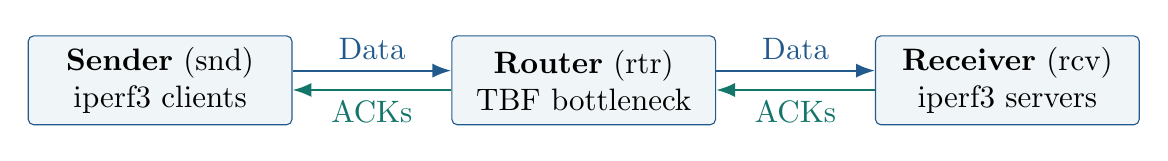
\begin{tikzpicture}[
  ns/.style={draw=flowblue,fill=diagramfill,rounded corners=2pt,
    minimum width=3.35cm,minimum height=1.13cm,align=center},
  >={Latex[length=2.4mm]},
  every node/.style={font=\reporttextsize}
]
\node[ns] (s) at (0,0) {\textbf{Sender} (snd)\\iperf3 clients};
\node[ns] (r) at (5.38,0) {\textbf{Router} (rtr)\\TBF bottleneck};
\node[ns] (d) at (10.76,0) {\textbf{Receiver} (rcv)\\iperf3 servers};
\draw[->,flowblue,thick] ([yshift=3.5pt]s.east) -- node[above]{Data} ([yshift=3.5pt]r.west);
\draw[->,flowblue,thick] ([yshift=3.5pt]r.east) -- node[above]{Data} ([yshift=3.5pt]d.west);
\draw[->,flowteal,thick] ([yshift=-3.5pt]d.west) -- node[below]{ACKs} ([yshift=-3.5pt]r.east);
\draw[->,flowteal,thick] ([yshift=-3.5pt]r.west) -- node[below]{ACKs} ([yshift=-3.5pt]s.east);
\end{tikzpicture}
\caption{Three namespaces connected by two virtual Ethernet pairs on one host. Loss injection was on sender egress in Part A. The router applied the 100 Mb/s bottleneck toward the receiver and 50 ms delay toward the sender.}
\label{fig:testbed}
\end{figure}

The links in Figure~\ref{fig:testbed} used a 1,500-byte MTU. The router's receiver-facing egress (\texttt{r1}) used a token bucket filter (TBF) at 100 Mb/s with a 4,542-byte burst and a byte-limited drop-tail queue. The nominal BDP was $100\,\mathrm{Mb/s}\times 0.050\,\mathrm{s}/8=625{,}000$ bytes, giving queue limits of 156,250, 625,000, and 2,500,000 bytes. On router egress toward the sender (\texttt{r0}), \texttt{netem} added 50 ms on the acknowledgement (ACK) path. In Part A, a separate \texttt{netem} on sender egress (\texttt{s0}) applied independent random packet loss before the TBF. It was also installed at 0\% loss to keep that queueing configuration consistent across Part A. Each \texttt{netem} used a 10,000-packet limit.

The source data were scripted transfers and kernel measurements in the isolated testbed. The 75 scheduled runs included every planned combination. Separate validation and pilot runs were used to calibrate the testbed and set the analysis windows.

\subsection{Work Procedure and Data Collection}

\textbf{Validation.} We disabled TSO, GSO, and GRO on all four virtual interfaces, disabled saving TCP destination metrics on the endpoints, and set the maximum TCP and system socket buffers to 16 MiB. In the initial validation, the drop counter showed 0.078\% loss with 0.5\% configured. Multi-segment socket buffers could still reach \texttt{netem} before software segmentation. We set \texttt{gso\_max\_segs} to 1 on the sender and receiver interfaces and repeated the checks. The measured loss was then 0.494\% (2,355 of 476,547 packets), within the tolerance of 0.1 percentage points. The other passing checks were idle RTT of 50.30 ms (within 1 ms of target), CUBIC receiver goodput of 95.37 Mb/s (at least 93), zero drops in the reverse-path delay queue, receiver-window limitation of 0.0\% in the CUBIC check (under 1\%), and maximum per-core CPU busy of 11.1\% (under 50\%).

\textbf{Pilots and schedule.} We ran one pilot competition at each queue size and inspected the per-flow goodput, queue backlog, and excess-RTT traces. The analysis used a 20 s warm-up for single flows and 60 s for competition. We ran Part A before Part B and shuffled conditions within each part using seed 2202. In Part B, separate iperf3 instances sent for 300 s each, with a 5 s start stagger. BBR started first in repetitions 1, 3, and 5, and CUBIC started first in repetitions 2 and 4, at each queue size.

\textbf{Per-run collection.} Before each run the driver recreated the queueing disciplines to reset counters, waited 5 s, and took 20 idle ping probes at 0.2 s intervals. It then started one iperf3 server per flow, collected socket and queue snapshots at nominal 100 ms intervals, pinged through the bottleneck at a requested 10 ms interval, and sampled per-core CPU usage each second. The receiver-side iperf3 JSON provided one-second payload byte counts. Sender-side \texttt{ss} recorded segment and retransmission counters. Router-side \texttt{tc} recorded queue backlog and drops. The driver saved TCP and queue counters before and after the transfer, the flow launch times, the actual congestion-control algorithms, and the software and condition identifiers.

\subsection{Data Analysis and Quality Assurance}

\textbf{Inclusion and windows.} The driver required error-free iperf3 results, receiver JSON, the requested congestion-control algorithm, and per-core CPU busy below 50\%. A Reno zero-injection attempt was rejected after a concurrent process drove a core to 100\% busy. Its valid retry was included. Across the 75 retained runs, the idle RTT medians ranged from 50.20 to 50.40 ms, the reverse-path delay queue recorded zero drops, and the maximum per-core CPU busy reached 21.8\% in Part A and 19.2\% in Part B.

The first client launch defined $t=0$ for each run. We used $(20,120]$ s for Part A and $(60,300]$ s for Part B. Receiver interval times were aligned using the corresponding client's recorded launch time. For continuous ping, the send time was estimated by subtracting RTT from the reply timestamp. Valid replies in the windows averaged approximately 66--80 per second across runs.

\textbf{Metrics.} For each flow, we summed receiver payload bytes from intervals ending in the analysis window, multiplied by eight, and divided by the summed durations of those intervals. This gave goodput in bits per second, which we report in Mb/s. A rate of 95.6 Mb/s is an approximate payload ceiling for 1,448 payload bytes per 1,514-byte frame at 100 Mb/s. For each flow's data socket, which we identified by its local port, we calculated $1{,}000\,\Delta\texttt{retrans}/\Delta\texttt{data\_segs\_out}$ using the first and last \texttt{ss} sample in the window.

We subtracted the run's median idle RTT from each returned probe's RTT and took P50, P95, and P99 of those differences. We also converted TBF backlog $b$ in bytes to a queueing-delay estimate $8b/(100\times 10^6)$ seconds. The two \texttt{netem} drop counters and the TBF drop counter distinguish drop locations. The ICMP probes measure path delay, including the queue shared by both flows in Part B.

For Part B, with $x_B$ and $x_C$ denoting per-flow goodputs over the window, aggregate goodput was $x_B+x_C$, BBR share was $x_B/(x_B+x_C)$, and Jain's index was $(x_B+x_C)^2/[2(x_B^2+x_C^2)]$ \cite{jain1984}. The index ranges from 0.5 for a one-sided allocation to 1 for an even split. We also checked BBR's share of received bytes across eight 30 s blocks. The rule for a settled run was an absolute difference of at most 0.10 between the first and last blocks. To check sensitivity to the window, we recomputed share, Jain's index, aggregate goodput, and P50 and P95 excess RTT over $(180,300]$ s.

\textbf{Comparison and reproducibility.} We summarized conditions with the median and interquartile interval $[Q_1,Q_3]$ across runs. The result plots show individual runs and medians. We compared the observed ranges and used selected two-sided Mann--Whitney $U$ tests with SciPy's exact method to assess separation between groups of five runs. We report unadjusted $p$ values alongside the magnitude of the contrasts. The Mathis reference uses $p$ as a probability, RTT of 50 ms, MSS of 1,448 bytes, and the random-loss constant 1.31 for one ACK per packet \cite{mathis1997}. Appendix~\ref{app:repro} identifies the archived data and Python analysis entry point.

\clearpage

\section{Results}

\subsection{RQ1. Single-Flow Response to Random Loss}

With 0\% injected loss, all three algorithms delivered above 93 Mb/s (Figure~\ref{fig:loss} and Table~\ref{tab:loss}). At 2\% loss, BBR delivered 89.6 Mb/s, or 96.0\% of its baseline median. CUBIC and Reno each fell below 2 Mb/s, retaining 1.7\% and 1.9\%, respectively. The 0\% and 2\% ranges were disjoint for each algorithm ($U=25$, $p=0.0079$ each).

\begin{figure}[!htbp]
\centering
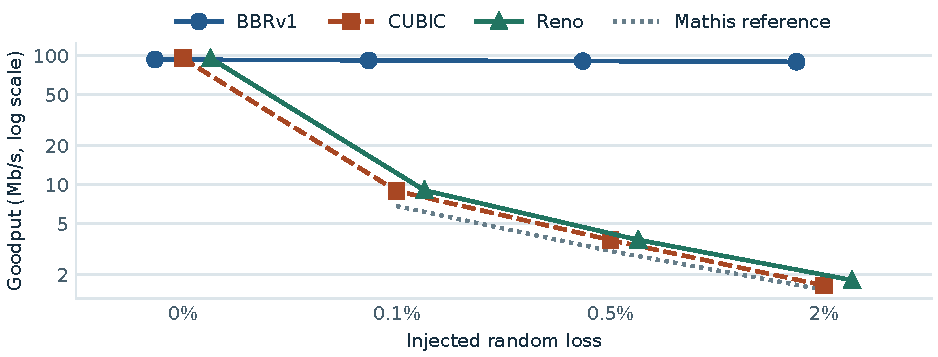
\includegraphics[width=\linewidth]{figures/loss-goodput.pdf}
\caption{Goodput by injected loss. Lines connect medians and the dotted line shows the Mathis reference.}
\label{fig:loss}
\end{figure}

The CUBIC--Reno median gap grew from 0.10 to 0.17 Mb/s between 0.1\% and 2\% loss. Their ranges overlapped at 0.1\% ($U=10$, $p=0.690$). At 2\%, every Reno run exceeded every CUBIC run ($U=0$, $p=0.0079$, CUBIC first). H1's retention thresholds were met, and its predicted narrowing of the gap was unsupported.

Retransmissions rose to about 19--20 per 1,000 data segments at 2\% loss. At 0\% injected loss, BBR, CUBIC, and Reno had median TBF drop counts of 0, 70, and 15, respectively. With injected loss, CUBIC and Reno's P95 excess RTT fell to about 0.1 ms. BBR's P95 fell from 12.3 to 7.6 ms across the sweep.

\begin{table}[!htbp]
\centering
\caption{Single-flow medians across five runs per condition. Goodput includes [Q1, Q3]. P50 and P95 refer to excess RTT.}
\label{tab:loss}
\begin{tabular}{@{}rlrrrr@{}}
\toprule
Loss (\%) & Algorithm & Goodput (Mb/s) & Retx/1,000 & P50 (ms) & P95 (ms) \\
\midrule
0 & BBRv1 & 93.37 [93.34, 93.44] & 0.00 & 1.3 & 12.3 \\
 & CUBIC & 95.37 [95.37, 95.39] & 0.08 & 34.7 & 48.3 \\
 & Reno & 95.35 [95.29, 95.35] & 0.02 & 30.1 & 47.1 \\
\addlinespace[2pt]
0.1 & BBRv1 & 91.97 [91.96, 91.97] & 1.01 & 0.3 & 11.4 \\
 & CUBIC & 8.92 [8.92, 9.27] & 0.97 & $-0.1$ & 0.1 \\
 & Reno & 9.03 [8.75, 10.21] & 1.03 & $-0.1$ & 0.1 \\
\addlinespace[2pt]
0.5 & BBRv1 & 90.71 [90.70, 90.80] & 5.03 & $-0.2$ & 8.8 \\
 & CUBIC & 3.71 [3.53, 3.72] & 5.04 & $-0.1$ & 0.1 \\
 & Reno & 3.72 [3.70, 3.87] & 5.49 & $-0.1$ & 0.1 \\
\addlinespace[2pt]
2 & BBRv1 & 89.60 [89.59, 89.66] & 19.97 & $-0.2$ & 7.6 \\
 & CUBIC & 1.65 [1.65, 1.75] & 18.80 & 0.0 & 0.1 \\
 & Reno & 1.81 [1.79, 1.87] & 20.03 & 0.0 & 0.1 \\
\bottomrule
\end{tabular}
\end{table}


\clearpage

\subsection{RQ2. Goodput Sharing Between BBR and CUBIC}

Median BBR share decreased across the three queue sizes from 96.8\% through 85.0\% to 43.5\% (Figure~\ref{fig:competition} and Table~\ref{tab:comp}). The three observed ranges were disjoint. All pairwise share comparisons gave $U=25$ and $p=0.0079$ when the smaller queue was entered first. The share crossed the even-split reference between the 1 and 4 BDP conditions, supporting H2. Jain's index increased from 0.533 to 0.984. For the last 120 s, the median shares were 96.7\%, 84.8\%, and 43.1\%. All 15 runs met the first-to-last block rule, with a maximum change of 8.5 percentage points.

\begin{figure}[!htbp]
\centering
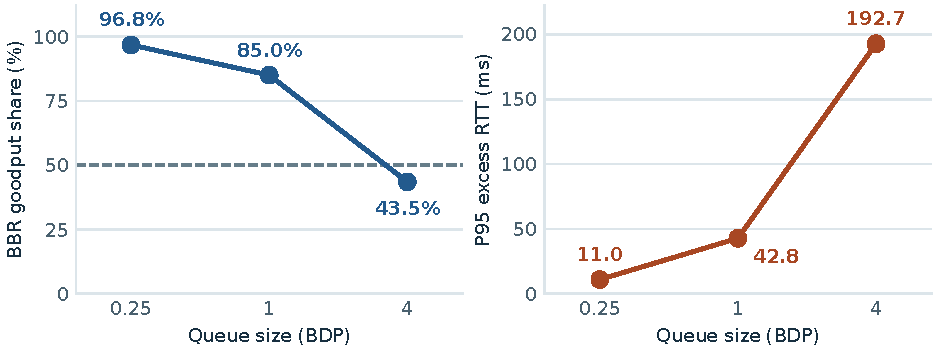
\includegraphics[width=\linewidth]{figures/competition.pdf}
\caption{BBR share and P95 excess RTT. Small markers show runs, large markers show medians, and the dashed line marks an even split.}
\label{fig:competition}
\end{figure}

\subsection{RQ3. Aggregate Goodput, Retransmissions, and Delay}

From 0.25 to 4 BDP, aggregate goodput rose by 3.1 Mb/s and P95 excess RTT rose from 11.0 to 192.7 ms. The other percentiles and the TBF backlog-based estimate also increased (Table~\ref{tab:comp}). The 4 BDP ranges for P50 and P95 were above both smaller queues ($U=0$, $p=0.0079$ each, smaller queue first).

\begin{table}[!htbp]
\centering
\caption{Competition results by queue size. Entries are medians of five run-level values, with interquartile intervals shown for the primary share, goodput, and P95 metrics.}
\label{tab:comp}
\vspace{4pt}
\begin{tabular}{@{}lrrr@{}}
\toprule
Metric & 0.25 BDP & 1 BDP & 4 BDP \\
\midrule
BBR goodput share (\%) & 96.8 [96.7, 96.8] & 85.0 [85.0, 85.1] & 43.5 [43.5, 44.8] \\
Jain's index & 0.533 & 0.671 & 0.984 \\
Aggregate goodput (Mb/s) & 92.14 [92.12, 92.14] & 93.21 [93.17, 93.24] & 95.28 [95.27, 95.28] \\
BBR retx/1,000 & 6.34 & 0.19 & 1.03 \\
CUBIC retx/1,000 & 14.24 & 1.05 & 0.90 \\
P50 excess RTT (ms) & 0.0 & 32.9 & 149.7 \\
P95 excess RTT (ms) & 11.0 [10.9, 11.0] & 42.8 [42.7, 43.0] & 192.7 [191.7, 193.7] \\
P99 excess RTT (ms) & 12.2 & 47.6 & 199.7 \\
Mean TBF delay (ms) & 1.9 & 31.5 & 147.6 \\
\bottomrule
\end{tabular}
\end{table}


For both flows, the 0.25 BDP retransmission rates exceeded both deeper queues ($U=25$, $p=0.0079$ for the four comparisons). Median TBF drops were 12,678, 617, and 1,934 as queue size increased. H3 was supported. The largest BBR share coincided with the most queue drops and the lowest excess RTT.

\clearpage

\section{Discussion}

\subsection{Interpretation and Answers to the Research Questions}

\textbf{RQ1.} The random-loss sweep separated BBR's goodput response from those of CUBIC and Reno. At 2\% loss, BBR maintained almost 90 Mb/s while retransmitting about 20 segments per 1,000 sent. Its pacing depends on estimated delivery rate and propagation RTT, allowing it to maintain a high rate while TCP recovers lost data \cite{cardwell2017,cao2019}. CUBIC and Reno reduced their windows in response to loss. The smaller windows are consistent with the near-idle delay percentiles and median zero TBF drops under injected loss. The Mathis reference gives roughly 9.6, 4.3, and 2.1 Mb/s for the three nonzero settings. Both loss-based algorithms followed the broad decline while delivering somewhat less than the reference. Its fixed-RTT and no-timeout assumptions make it an approximate comparison, especially at 2\% \cite{mathis1997}. The small CUBIC--Reno gap changed in the opposite direction from the prediction. With five runs per condition, the evidence supports a similarly large degradation for both algorithms on this path.

\textbf{RQ2.} The queue sweep shifted the split from strong BBR dominance to a slight CUBIC advantage. In the shallow queue, the high TBF drop count and CUBIC retransmission rate are consistent with CUBIC repeatedly reducing its window while BBR continued to probe. In the deep queue, CUBIC had room to increase its window and maintain a large backlog. This pattern agrees with the direction observed by Jaeger et al. and with Ware et al.'s explanation linking BBRv1's share to its inflight limit \cite{jaeger2019,ware2019}. The present experiment varied the queue at three points and measured the resulting split. Intermediate queue settings and direct validation of the inflight mechanism remain open.

\textbf{RQ3.} Similar aggregate goodputs concealed very different operating conditions for the two flows and for other traffic using the queue. Moving from 0.25 to 4 BDP improved the average split and reduced retransmissions relative to the shallow queue, but added 181.7 ms to P95 excess RTT. The backlog-based delay rose from 1.9 to 147.6 ms, consistent with persistent queueing in the deep condition. The 1 BDP queue had the fewest TBF drops and the lowest BBR retransmission rate, but still gave BBR 85.0\% of delivered data. These findings give a concrete trade-off among sharing, delay, and loss for the queue sizes tested.

\subsection{Validity, Limitations, and Generalizability}

Resetting the queues and interleaving conditions within each part reduced differences due to run history and time of day. The validation run, stable idle RTT, and CPU samples support the rate and loss settings despite the move to WSL2. One-second CPU averages can miss short scheduling delays, and the effective ping sampling rate was below the requested rate. Differences of a few tenths of a millisecond around zero excess RTT are comparable to idle-RTT variation. The comparison between the deeper and shallower competition queues is much larger than this variation.

Excess-RTT percentiles use successful ICMP replies. Drops can remove probes that encounter a full queue, and ping RTT includes timing effects outside the TBF. The backlog samples corroborate the direction of the delay change, with a different sampling interval and estimand. The 30 s block rule detects large changes between the endpoints of the competition window. It can miss shorter oscillations, and Jain's index computed from mean rates can mask temporary starvation even when the window-average split is close to equal \cite{jaeger2019}.

The 75 runs cover the chosen conditions on one emulated host. With five runs per condition, the exact rank tests have only 252 possible allocations and a minimum two-sided $p$ value of $0.0079$ for untied data. The comparisons were unadjusted for multiplicity and have limited precision for smaller contrasts. Alternating the start order exposed each queue to both launch orders and left a three-to-two imbalance. The first-to-last comparison and the last-120-s analysis support the reported ordering, while simultaneous and differently staggered arrivals could lead to different rates.

The findings apply to long-lived Linux BBRv1, CUBIC, and Reno flows on one drop-tail path with fixed capacity and RTT. Injected loss was independent and on the forward path. Deployments with bursty loss, RTT asymmetry, multiple flows, short transfers, or active queue management can produce other results. BBR versions differ in their coexistence behavior \cite{sarpkaya2025}. The three tested queue sizes bound the interval over which the larger share changed hands.

\subsection{Ethics, Societal Aspects, and Sustainability}

All test transfers and probes stayed within three local namespaces. The isolated setup avoided collecting personal communications and sending bulk test traffic over shared networks. Recording the rejected attempt, validation failure, and full condition set makes the measurement decisions inspectable.

A shared access link can serve bulk transfers and delay-sensitive activities such as calls. In the shallow-queue condition, the same link delivered high aggregate goodput while one of the competing flows received just over 3\% of the payload rate. In the deep condition, sharing improved while the upper tail of delay grew. Both outcomes matter to operators and users. The equal-throughput reference concerns two sustained flows with equal base RTT, whereas users may have multiple connections and different latency needs.

The measurements used an existing host and software emulation. Retransmissions represent additional transmissions for the amount delivered and can increase the resources required to carry traffic. We measured segment counts, goodput, and delay. Energy per delivered byte would require power measurements and explicit accounting for the test host and network equipment.

\subsection{Implications and Future Work}

On this path, aggregate goodput alone would have hidden the practical difference among the three queue settings. A deployment evaluation should consider per-flow sharing, retransmissions, and delay percentiles together. The immediate follow-up is to test intermediate queue sizes between 1 and 4 BDP with more balanced start-order repeats and longer overlaps. This would locate the change in the split and quantify variation under both launch orders. Repeating the comparison on bare-metal Linux with a newer BBR version and an active queue-management configuration would test whether a more even allocation is possible with less delay.

\section{Conclusion}

On the emulated 100 Mb/s, 50 ms path, BBRv1 retained 96.0\% of baseline goodput at 2\% injected loss, while CUBIC and Reno each retained less than 2\%. BBRv1's median share against CUBIC fell from 96.8\% at 0.25 BDP to 43.5\% at 4 BDP. Aggregate goodput increased by only 3.1 Mb/s across those endpoints, while the deepest queue added substantially more tail delay and the shallowest produced the most retransmissions for both flows. The experiment shows why algorithm and queue comparisons on a shared link need to report delivered rate, sharing, and delay together.

\clearpage
\bibliographystyle{myIEEEtran}
\bibliography{II2202_Group5_References}

\clearpage
\appendix
\section{Reproducibility Details}
\label{app:repro}

The archive is \href{https://github.com/icannotworkoutaname/ii2202-cc-experiment/tree/a49b86cd009d5e085079719bca25fa4a075c03f3}{\texttt{ii2202-cc-experiment}} at commit \texttt{a49b86c}. The testbed files used for measurement are in \texttt{5a18ab9}. Some archived run metadata retain the commit ID from before its message was edited. The repository's \texttt{HANDOFF.md} documents that provenance.

\begin{tabularx}{\linewidth}{@{}>{\raggedright\arraybackslash}p{0.37\linewidth}X@{}}
\toprule
Archive location & Contents \\
\midrule
\texttt{testbed/params.json} & Condition matrix, schedule seed, time limits, sampler intervals, and CPU cutoff. \\
\texttt{docs/host\_*} & Kernel, processor, congestion-control module, and interface settings. \\
\texttt{validation/} and \texttt{pilot/} & Preflight checks, initial loss-calibration failure, corrected checks, and pilot traces. \\
\texttt{runs/schedule.csv} and \texttt{runs/run\_log.csv} & Planned execution order and recorded attempts, including the rejected run. \\
\texttt{runs/A\_*}, \texttt{runs/B\_*} & Run metadata, iperf3 output, socket and queue samples, ping replies, and CPU measurements. \\
\texttt{analysis/out/} & Per-run metrics, summaries, tests, share-window checks, and figures. \\
\bottomrule
\end{tabularx}

Use Python 3.10 or later with the packages in \texttt{requirements.txt}. Run the command below from the experiment checkout to recompute the summaries in a separate directory.

{\ttfamily python3 analysis/analyze.py --runs runs --out /tmp/ii2202-analysis\par}

The reanalysis matched all six archived CSV tables numerically and both archived LaTeX summary tables exactly. The condition totals and actual TCP algorithms were cross-checked against the schedule and each run's metadata.

\end{document}
